\documentclass{IOS-Book-Article}

\usepackage{graphicx}

\usepackage[square,numbers,sort]{natbib}

\usepackage{booktabs}
\usepackage{multirow}

\usepackage{color}
\usepackage[pdfusetitle]{hyperref}
% http://colorschemedesigner.com/#4o42FfqublRMS
\definecolor{linkcolor}{RGB}{66, 54, 122}
\definecolor{citecolor}{RGB}{84, 141, 100}
\definecolor{urlcolor}{RGB}{168, 70, 67}
\hypersetup{
  colorlinks=true,
  linkcolor=linkcolor,
  citecolor=citecolor,
  urlcolor=urlcolor,
}

\usepackage{soul}
\definecolor{hlcolor}{RGB}{255, 221, 163}
\sethlcolor{hlcolor}
\usepackage{mathptmx}

%\usepackage{times}
%\normalfont
\usepackage[T1]{fontenc}
%\usepackage[mtplusscr,mtbold]{mathtime}
%

\newcommand{\sn}[1]{\href{https://twitter.com/#1}{\texttt{@#1}}}

\begin{document}
\begin{frontmatter}              % The preamble begins here.

%\pretitle{Pretitle}
\title{LV2}
\runningtitle{LV2}
%\subtitle{Subtitle}

\author[A]{\fnms{Anonymous} \snm{Submission}%
\thanks{Corresponding Author: Book Production Manager, IOS Press, Nieuwe Hemweg 6B,
1013 BG Amsterdam, The Netherlands; E-mail:
bookproduction@iospress.nl.}}
%\author[B]{\fnms{Second} \snm{Author}}
%and
%\author[B]{\fnms{Third} \snm{Author}


%\runningauthor{B.P. Manager et al.}
\address[A]{Confidential Review Copy, Do Not Distribute}
%\address[B]{Short Affiliation of Second Author and Third Author}

%\begin{abstract}
%
%\end{abstract}

\begin{keyword}
Corpus Linguistics \sep Latvian \sep Russian \sep English
\end{keyword}
\end{frontmatter}

\thispagestyle{empty}
\pagestyle{empty}

\section*{Introduction}

This paper presents a multilingual, location-anchored corpus of tweets from Latvia. The main challenge of collecting a socially representative corpus from this country is that several languages are used there: Latvian, the main communication language, Russian, the language of the largest minority in Latvia, and English.

%%%%%%%%%
% Problem
%%%%%%%%%
%There are several challenges of building a tweet collection that adequately represents language use in the country.
%
Building a monolingual Latvian collection could be done by harvesting tweets that contain indicative Latvian words which do not present in other languages, similarly to how it is done for Dutch \cite{sang2013}. However, such an approach is not suitable for tweets in Russian and English, as these languages are widely used outside of Latvia.
%
For the same reason, a TREC-like collection building approach \cite{lin2016overview} of filtering the publicly available stream of tweets by language would not work.
%
A tweet collection based on a curated list of users \cite{SANVICENTE16.465} is effective, but extra care must be taken as tracking personal accounts might be problematic due to privacy concerns.
%
A geo-location based collection produces representative results \cite{milajevs:2017:BUCC}. It is not biased linguistically because it is not based on a list of keywords. It is not biased thematically because it is not based on a list of users. However, a large number of tweets is not geo-located, which makes retrieval incomplete.

%%%%%%%%
% Method
%%%%%%%%
To keep a balance between privacy and objectivity maximizing completeness, this work applies a hybrid approach by combining a geo-location based collection procedure with tracking a curated list of users. To minimize privacy issues, only accounts of organizations and public figures are tracked.

%%%%%%%%%
% Results
%%%%%%%%%

%%%%%%%%%%%%%
% So, what...
%%%%%%%%%%%%%

\section{Data collection}
\label{sec:data-collection}

Over the period from 15 April 2017 to \hl{19 April 2018} the initial set of \hl{1\,685\,048} tweets was collected from the \texttt{POST status/filter} endpoint of the Twitter Streaming API.\footnotemark{}
%
\footnotetext{\url{https://developer.twitter.com/en/docs/tweets/filter-realtime/api-reference/post-statuses-filter}}
%
The \texttt{locations} parameter was set to the bounding box of Riga, the capital of Latvia.\footnotemark{}
%
\footnotetext{The coordinates of the bounding box are \texttt{23.9325829, 56.8570671, 24.3247299, 57.0859184}.}
%
In addition to the location, \hl{420} accounts were tracked. \hl{The whole list of screen names together with user ID is available in the supplement.}

To comply with Twitter's terms of service, on \hl{19 April 2018}, the raw tweet data was redownloaded (or rehydrated) to get rid of deleted tweets. The tweets that originated a retweet were added to the collection. Also, we have noticed a large number of tweets that came from Sweden (probably because of the imprecise \texttt{locations} parameter value), so the tweets which location country code was \texttt{SE} were omitted. This resulted in \hl{1\,133\,812} tweets that formed the final collection presented here.

\section{Twitter users}
\label{sec:global-analysis}

\begin{table}
  \centering
  \begin{tabular}{lrllrlrlrlrl}
\toprule
lang & total\_count & total\_share & tracked\_source\_share & \multicolumn{2}{l}{lv} & \multicolumn{2}{l}{ru} & \multicolumn{2}{l}{en} & other\_lang\_count & other\_lang\_share \\
{} & source\_lang\_count & source\_lang\_share & source\_lang\_count & source\_lang\_share & source\_lang\_count & \multicolumn{3}{l}{source\_lang\_share} \\
source\_pretty       &             &             &                      &                   &                   &                   &                   &                   &                   &                  &                  \\
\midrule
Twitter Web Client  &      465845 &       34.1\% &                52.4\% &            386342 &             82.9\% &             14718 &              3.2\% &             38715 &              8.3\% &            26070 &             5.6\% \\
Twitter for Android &      227534 &       16.7\% &                 8.3\% &            153578 &             67.5\% &             22351 &              9.8\% &             34632 &             15.2\% &            16973 &             7.5\% \\
Twitter for iPhone  &      205280 &       15.0\% &                14.0\% &            123388 &             60.1\% &             32796 &             16.0\% &             31829 &             15.5\% &            17267 &             8.4\% \\
TweetDeck           &      104345 &        7.6\% &                91.7\% &            102261 &             98.0\% &                75 &              0.1\% &              1470 &              1.4\% &              539 &             0.5\% \\
TVNET Login         &       57733 &        4.2\% &                96.7\% &             26231 &             45.4\% &             30826 &             53.4\% &                23 &              0.0\% &              653 &             1.1\% \\
dlvr.it             &       45337 &        3.3\% &                98.4\% &             44806 &             98.8\% &               134 &              0.3\% &               129 &              0.3\% &              268 &             0.6\% \\
Facebook            &       36327 &        2.7\% &                95.1\% &             13741 &             37.8\% &             20833 &             57.3\% &               450 &              1.2\% &             1303 &             3.6\% \\
Foursquare          &       30708 &        2.3\% &                 0.0\% &             24300 &             79.1\% &               220 &              0.7\% &              1881 &              6.1\% &             4307 &            14.0\% \\
Instagram           &       24654 &        1.8\% &                 1.7\% &              8801 &             35.7\% &              2450 &              9.9\% &              8164 &             33.1\% &             5239 &            21.3\% \\
SKATIES             &       22798 &        1.7\% &                98.0\% &             22782 &             99.9\% &                 0 &                 0 &                 0 &                 0 &               16 &             0.1\% \\
\bottomrule
\end{tabular}
  
  \caption{Global statistics.}
\end{table}

On average, about \hl{3\,200} tweets were collected per day, which is more than \hl{1\,500} by the geo-location based technique in \cite{milajevs:2017:BUCC}. Most of the tweets came from the official Twitter clients for Web, Android or iPhone. Together these clients contributed more than 60\% of all collected tweets, refer to Table~\ref{tab:source_counts} for more details.

The twitter web client is used by both: the general public and media companies. The top 5 of most active accounts consists only of tracked Latvian media accounts: \sn{DienaLV}, a newspaper, \sn{LA\_lv}, another newspaper, \sn{JaunsLV}, a media portal, \sn{TV3\_Play}, a TV channel, and \sn{dblv}, a newspaper.


Notably, for mobile clients, the majority of tweets comes from the general public, because they are either geo-located or mention a tracked account. The number of tweets coming from tracked accounts, \hl{that are mostly media}, is lower for Android \hl{(8.5\%)} than for iPhone \hl{(13.5\%)}. The difference can be explained by the fact, that all top 5 Android users are personal accounts, while for iPhone there are only 2 personal accounts in the top 5. \sn{TV3zinas}, a news account of a TV channel, tweets the most from iPhone. \sn{Lattelecom}, a telecommunication company, is the second most active iPhone user. \sn{AstrologiLv} writes about astrology and is the fourth most active iPhone user. All three accounts tweet exclusively in Latvian and were tracked during corpus collection.

Client applications that produce tweets mostly from tracked accounts are used by the media. For the TweetDeck, TVNET Login, dlvr.it and SKATIES client applications the top 5 users are tracked media accounts that write dominantly in Latvian. The exceptions are a business account \sn{Kompresori} that was not tracked and tweets in three languages: Latvian, Russian and English, \sn{RusApollo} and \sn{TVNET\_rus} who tweet identical content exclusively in Russian, and \sn{SejasLV}, an exclusively Latvian account writing about celebrities, which was not tracked.

TweetDeck is used by \sn{DelfiLV}, a major media portal, \sn{LV\_Portals}, an account run by the official government gazette of the Republic of Latvia, \sn{lsmlv}, an account of a publicly funded radio and television organization (LSM), \sn{ltvzinas}, the news account of Latvian Television, \sn{RietumuRadio}, a radio station. 

TVNET is a media company that controls several media portals. The most active accounts that use their application are \sn{TVnet\_portals}, \sn{RusApollo}, \sn{TVnet\_rus}, \sn{SportsTVNET}, and \sn{SejasLV}.

The tweet delivery service \texttt{dlvr.it} is used by the newspaper \sn{nralv} and their sport portal \sn{Sportacentrs}, the photo account of the national news agency (LETA) \sn{letafoto}, \sn{Kompresori} and the sport account of Latvian Television \sn{ltvsports}.

SKATIES delivers video content from several sources. The most active accounts are \sn{skatieslatvija}, \sn{lnt\_lv}, \sn{tv3lv}, \sn{BezTabuTV3} and \sn{TV3Zinas}.

Some tweets come from social media networks. Facebook content mostly comes from tracked media accounts. The top 5 most active users are: \sn{mixnews\_lv}, the Russian edition of a media portal, \sn{Otkrito}, also the Russian edition of \sn{JaunsLV}, \sn{labdienlv}, \sn{ekonimikalv} and \sn{nozare}, all three belonging to one Latvian media portal. The fact that Russian accounts are not active among other clients might suggest that Russian content is not spread via Twitter, but via Facebook.

The content that comes form Foursquare and Instagram is created by the general public.

There is a clear pattern that mobile clients are used by personal accounts, while media companies set up a special solution to deliver tweets, probably, integrating it with their content delivery systems or simply using a web client from an office machine.

\section{Language}
\label{sec:language}

Latvian is the dominant language: \hl{880\,351 (74\%)} tweets are written in it.\footnotemark{} There are \hl{12\,505 (11\%)} tweets in Russian, \hl{116203 (10\%)} in English and \hl{66\,969 (6\%)} in other languages. Figure~\ref{fig:rehydrated-tweets-count-by-day} shows the tweet volume over time.

\footnotetext{Twitter labels tweets with the language they are written in.}

Latvian dominates almost in every client application. Tweets coming from Foursquare are labeled as Latvian in \hl{78\%} cases (see Table~\ref{tab:source_counts}), that might be due to Latvian location names.

Russian tweets constitute of more then half tweets coming from TVNET, where its share is \hl{52\%} while Latvian is \hl{46.3\%}, and from Facebook, where the two most active users are Russian madia.

A lot of English content is coming form Instagram (\hl{32.9\%}), that might be due to the dominance of hashtags over other text. Also, there are many tweets labeled as written in other languages that come from Foursquare and Instagram. As Instagram posts are more likely to contain hashtags and Foursqure tweets contain location names, tweets should not be assigned a single language label, but instead be labeled as written in several languages.

\section{Topics}
\label{sec:topics}

To investigate the collection further nine topics of interests were defined. The collection was manually searched using keywords to get relevant tweets. The topics are
\begin{itemize}
\item \texttt{LV001: Winter} Everything about winter. The relevant tweets are mostly about the weather, the pictures of snow and driving conditions.
\item \texttt{LV002: Mel\=anijas hronika} Mel\=anijas hronika is a Latvian movie that was selected for Foreign-Language Category for Oscars.
\item \texttt{LV003: Refugees} A broad topic about refugee crisis in Europe, attitude to immigration and immigrants.
\item \texttt{LV004: Dv\=eese\c{l}u putenis} A Latvian movie that is currently in production.
\item \texttt{LV005: Hockey} Ice hockey related tweets.
\item \texttt{LV006: Christmas} Christmas.
\item \texttt{LV007: New Year} New Year.
\item \texttt{LV008: Olympics} Tweets about the Olympic games and the Latvian team.
\item \texttt{LV009: Brexit} Brexit.
\end{itemize}




\begin{figure}
\centering

\caption{Tweet volume by day per language averaged over a rolling window of 7 days.}

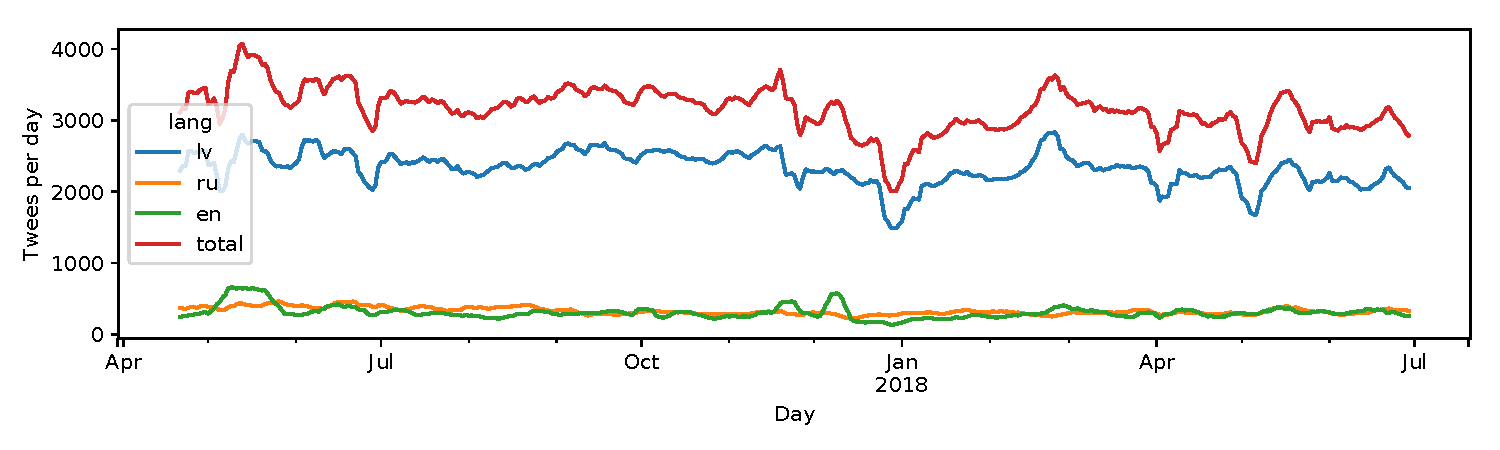
\includegraphics[width=\textwidth]{supplement/rehydrated_tweets_count_by_day.pdf}

\label{fig:rehydrated-tweets-count-by-day}
\end{figure}

%%% Local Variables:
%%% mode: latex
%%% TeX-master: "../paper.tex"
%%% End:

\bibliographystyle{unsrtnat}
\bibliography{references,dmilajevs_publications}

\end{document}
